\documentclass{article}
\usepackage{amsmath, amssymb, bm}
\usepackage{braket}

% Enhanced packages for better document structure
\usepackage{titlesec}
\usepackage{tocloft}
\usepackage{amsthm}
\usepackage{thmtools}
\usepackage{mdframed}
\usepackage{enumitem}
\usepackage{geometry}
\usepackage{xcolor}
\usepackage{tikz} % Added for circuit diagrams

% Set better margins
\geometry{margin=1in}

% Configure theorem-like environments
\newtheorem{theorem}{Theorem}[subsection]
\newtheorem{definition}[theorem]{Definition}
\newtheorem{example}[theorem]{Example}

% Define a nice box for important concepts
\newmdenv[
  linewidth=0.5pt,
  skipabove=1em,
  skipbelow=1em,
  backgroundcolor=gray!10,
  innerleftmargin=5pt,
  innerrightmargin=5pt,
  innertopmargin=5pt,
  innerbottommargin=5pt
]{conceptbox}

% Configure section formatting for chapters
\titleformat{\section}
  {\LARGE\bfseries}{\thesection.}{1em}{\MakeUppercase}
\titlespacing*{\section}{0pt}{3.5ex plus 1ex minus .2ex}{2.3ex plus .2ex}

% Configure subsection and subsubsection formatting
\titleformat{\subsection}
  {\Large\bfseries}{\thesubsection}{1em}{}
\titleformat{\subsubsection}
  {\large\bfseries}{\thesubsubsection}{1em}{}

% Configure spacing
\titlespacing*{\subsection}{0pt}{3.25ex plus 1ex minus .2ex}{1.5ex plus .2ex}
\titlespacing*{\subsubsection}{0pt}{3.25ex plus 1ex minus .2ex}{1.5ex plus .2ex}

% Configure list spacing
\setlist{itemsep=0.5em}

% Configure TOC depth and formatting
\setcounter{tocdepth}{3}
\renewcommand{\cftsecfont}{\Large\bfseries}
\renewcommand{\cftsecpagefont}{\bfseries}
\renewcommand{\cftsubsecindent}{2em}
\renewcommand{\cftsubsubsecindent}{4em}

\title{Quantum Computing Fundamentals}
\author{PHYS 370}
\date{Spring 2025}

\begin{document}
\maketitle

\newpage
\tableofcontents
\newpage

\section{Lecture 3: Quantum Gates and Circuits}
\subsubsection*{January 29, 2025}

\subsection{Matrix Representation of Quantum Gates}
\begin{conceptbox}
In quantum computing, the state of an \(n\)-qubit system is represented by a \(2^n\)-dimensional vector. Quantum gates are represented by \(2^n \times 2^n\) unitary matrices. A six-qubit quantum gate must be represented by a \(64 \times 64\) unitary matrix. The unitary condition:
\[
U^{\dagger}U = U U^{\dagger} = I,
\]
where \(U^{\dagger}\) is the Hermitian conjugate (conjugate transpose) of \(U\).
\end{conceptbox}

\subsection{Pauli Matrices as Quantum Gates}
\begin{definition}[Pauli Matrices]
The Pauli matrices (\(X, Y, Z\)) are fundamental single-qubit gates:
\begin{align*}
X & = \begin{bmatrix} 0 & 1 \\ 1 & 0 \end{bmatrix} \quad \text{(Bit-flip gate)} \\
Y & = \begin{bmatrix} 0 & -i \\ i & 0 \end{bmatrix} \quad \text{(Bit \& Phase-flip)} \\
Z & = \begin{bmatrix} 1 & 0 \\ 0 & -1 \end{bmatrix} \quad \text{(Phase-flip gate)}
\end{align*}
These matrices are unitary (\(U^{\dagger} = U^{-1}\)) and Hermitian (\(U = U^{\dagger}\)), ensuring valid quantum operations.
\end{definition}

\subsection{Controlled-NOT (CNOT) Gate}
\begin{definition}[CNOT Gate]
The CNOT gate acts on two qubits, with one acting as a control and the other as a target. It performs a NOT operation on the target if and only if the control qubit is \(|1\rangle\).
\end{definition}

\begin{example}[CNOT Matrix Representation]
\[
\text{CNOT} = \begin{bmatrix} 1 & 0 & 0 & 0 \\ 0 & 1 & 0 & 0 \\ 0 & 0 & 0 & 1 \\ 0 & 0 & 1 & 0 \end{bmatrix}
\]
\end{example}

\begin{theorem}[CNOT Action]
Using Dirac notation, its action is:
\begin{align*}
|00\rangle &\to |00\rangle \\
|01\rangle &\to |01\rangle \\
|10\rangle &\to |11\rangle \quad \text{(flips target qubit)} \\
|11\rangle &\to |10\rangle
\end{align*}
\end{theorem}

\subsection{Hadamard Gate and Bell State Generation}
\begin{definition}[Hadamard Gate]
The Hadamard gate (\(H\)) puts a qubit into an equal superposition:
\[
H = \frac{1}{\sqrt{2}} \begin{bmatrix} 1 & 1 \\ 1 & -1 \end{bmatrix}
\]
\end{definition}

\begin{example}[Bell State]
A fundamental Bell state:
\[
|\beta_{00}\rangle = \frac{|00\rangle + |11\rangle}{\sqrt{2}}
\]
\end{example}

The circuit construction consists of:
\begin{enumerate}
    \item Applying \(H\) to the first qubit.
    \item Applying CNOT, with the first qubit as the control.
    \item H turns the \(|0\rangle\) into \(|+\rangle\) and \(|1\rangle\) into \(|-\rangle\)
\end{enumerate}

\subsection{Quantum Circuit Representation}
\begin{itemize}
    \item Wires represent qubits and their evolution through time, not physical movement.
    \item Single-qubit gates (\(X, H, Z\), etc.) act on one qubit.
    \item Multi-qubit gates (CNOT, Toffoli) involve entanglement.
    \item Measurement collapses the quantum state and is usually represented by an encircled \(M\) in diagrams.
\end{itemize}

\subsection{Controlled Gates and Universal Quantum Gates}
\begin{definition}[Controlled Gates]
Controlled gates allow conditional operations:
\end{definition}

\begin{itemize}
    \item Controlled-Z (CZ): Applies a \(Z\) gate to the target when control is \(|1\rangle\).
    \item Controlled-Hadamard (CH): Applies \(H\) to the target when control is \(|1\rangle\).
    \item Toffoli Gate (CCNOT): Uses two control qubits and one target, flipping the target only when both controls are \(|1\rangle\).
    \item Fredkin Gate (CSWAP): Swaps two qubits based on a control qubit.
\end{itemize}

\subsection{Gate Decomposition}
\begin{conceptbox}
Complex multi-qubit gates can be decomposed into single-qubit gates and CNOTs. Example: Controlled-\(U\) decomposition replaces a controlled-\(U\) gate with a sequence of CNOTs and single-qubit rotations, used for efficient quantum circuit optimization.
\end{conceptbox}

\subsection{No-Cloning Theorem and Quantum Cloning}
\begin{theorem}[No-Cloning]
The CNOT gate cannot clone an arbitrary quantum state due to the no-cloning theorem. Example: Trying to copy \(\alpha|0\rangle + \beta|1\rangle\) results in entanglement, not an identical copy. Some specific states, like \(|0\rangle\) or \(|1\rangle\), can be cloned, but arbitrary superpositions cannot.
\end{theorem}

\subsection{Multi Qubit or Composite States}
\begin{definition}[Multi-Qubit States]
\begin{itemize}
    \item An n-qubit diagram will have n wires/lines
    \item Tensor product state
    \item entangled states (Bell) \(\alpha|0\rangle + \beta|1\rangle\)  and \(|1\rangle\) \textbf{bold}
\end{itemize}
\end{definition}

\subsubsection{Tensor Product State}
\begin{definition}[Tensor Product]
A tensor product state is a product of single-qubit states. An example of this is 2 \(|0\rangle\) qubits in tensor product state: \(|0\rangle \otimes |0\rangle = |0\rangle |0\rangle = |00\rangle\)
\end{definition}

\begin{example}[Matrix Representations]
\begin{itemize}
    \item \(|00\rangle = \begin{bmatrix} 1 \\ 0 \\ 0 \\ 0 \end{bmatrix}\)
    \item \(|11\rangle = \begin{bmatrix} 0 \\ 0 \\ 0 \\ 1 \end{bmatrix}\)
    \item \(|01\rangle = \begin{bmatrix} 0 \\ 1 \\ 0 \\ 0 \end{bmatrix}\)
\end{itemize}
\end{example}

\subsubsection{Bell States}
\begin{conceptbox}
Bell states are quintessential entangled 2-qubit states. Pauli exclusion principle states that no two fermions can occupy the same quantum state. So if you have one electron spin up and one spin down, the sign is minus. Also, a cheat sheet for signs is any state with a 1 first is minus, and 0 first is plus.
\end{conceptbox}

\paragraph{Bell State 1} \(|\beta_{00}\rangle = \frac{|00\rangle + |11\rangle}{\sqrt{2}}\)
\begin{itemize}
    \item In this state you know the bit on the right by measuring the bit on the left.
    \item If the left bit is \(|0\rangle\) then the right bit is \(|0\rangle\)
    \item If the left bit is \(|1\rangle\) then the right bit is \(|1\rangle\)
    \item This is a Bell state because it is an entangled state.
\end{itemize}

\paragraph{Bell State 2} \(|\beta_{01}\rangle = \frac{|01\rangle + |10\rangle}{\sqrt{2}}\)
\begin{itemize}
    \item In this state you know the bit on the left by measuring the bit on the right.
    \item If the right bit is \(|0\rangle\) then the left bit is \(|1\rangle\)
    \item If the right bit is \(|1\rangle\) then the left bit is \(|0\rangle\)
    \item This is a Bell state because it is an entangled state.
\end{itemize}

\paragraph{Bell State 3} \(|\beta_{10}\rangle = \frac{|00\rangle - |11\rangle}{\sqrt{2}}\)
\begin{itemize}
    \item In this state you know the bit on the right by measuring the bit on the left.
    \item If the left bit is \(|0\rangle\) then the right bit is \(|1\rangle\)
    \item If the left bit is \(|1\rangle\) then the right bit is \(|0\rangle\)
    \item This is a Bell state because it is an entangled state.
\end{itemize}

\paragraph{Bell State 4} \(|\beta_{11}\rangle = \frac{|01\rangle - |10\rangle}{\sqrt{2}}\)
\begin{itemize}
    \item In this state you know the bit on the left by measuring the bit on the right.
    \item If the right bit is \(|0\rangle\) then the left bit is \(|1\rangle\)
    \item If the right bit is \(|1\rangle\) then the left bit is \(|0\rangle\)
    \item This is a Bell state because it is an entangled state.
\end{itemize}

\subsubsection{CNOT 2-qubit Operator}
\begin{definition}[CNOT 2-qubit Operator]
To make Bell states we need the CNOT 2-qubit operator. Given by:
\[
\text{CNOT} = \begin{bmatrix} 1 & 0 & 0 & 0 \\ 0 & 1 & 0 & 0 \\ 0 & 0 & 0 & 1 \\ 0 & 0 & 1 & 0 \end{bmatrix}
\]
\end{definition}

\begin{itemize}
    \item If the control qubit is \(|0\rangle\) then the target qubit is unchanged.
    \item If the control qubit is \(|1\rangle\) then the target qubit is flipped.
\end{itemize}

\subsection{Key Takeaways for Class Questions}
\begin{conceptbox}
\begin{itemize}
    \item What size matrix represents an \(n\)-qubit gate? \(2^n \times 2^n\) unitary matrix.
    \item Why are Pauli matrices quantum gates? They are unitary and Hermitian.
    \item What is the role of CNOT? Flips the target qubit if the control is \(|1\rangle\).
    \item How does Hadamard create superposition? Equal probability of \(|0\rangle\) and \(|1\rangle\).
    \item What do wires in a circuit mean? Time evolution of a quantum state.
    \item Can quantum states be cloned? No, due to the no-cloning theorem.
\end{itemize}
\end{conceptbox}

\newpage
\section{Lecture 4: Advanced Quantum Operations}
\subsubsection*{February 3, 2025}

\subsection{Checkpoint: Quiz Questions and Answers}
\begin{conceptbox}
\textbf{Key Questions and Answers:}
\begin{enumerate}
    \item \textbf{Q: What is the problem with trying to make copies of quantum data?} \\
    \textbf{A:} There is no unitary operator that exists which could be used to clone arbitrary quantum states, and so it simply isn't possible.
    
    \item \textbf{Q: In the teleportation example with Alice and Bob, why is the overall interaction remarkable?} \\
    \textbf{A:} Because a measurement on Alice's end seemingly 'caused' a change on Bob's end across space and time through no classical communication, only quantum.
    
    \item \textbf{Q: Why is it necessary for Alice to make a measurement during the teleportation process?} \\
    \textbf{A:} Because the very act of measurement will 'collapse' the unknown state into one of the other four possible states, depending on what Alice measures.
\end{enumerate}
\end{conceptbox}

\subsection{No-Cloning Theorem}
\begin{definition}[No-Cloning Theorem]
It is impossible to create an identical copy of an arbitrary unknown quantum state. There is no \underline{universal} unitary operator that will allow us to create a copy of an \underline{arbitrary} quantum state.
\end{definition}

\begin{theorem}[Mathematical Explanation]
Suppose a unitary operation \(U\) could clone states:
\[
U(|\psi\rangle \otimes |\chi\rangle) = |\psi\rangle \otimes |\psi\rangle
\]
\[
U(|\phi\rangle \otimes |\chi\rangle) = |\phi\rangle \otimes |\phi\rangle
\]
By taking the inner product and using the properties of unitarity, we reach a contradiction. This means cloning only works for orthogonal states but not for arbitrary quantum states.
\end{theorem}

\subsection{Quantum Teleportation}
\begin{definition}[Quantum Teleportation]
Quantum teleportation allows the transfer of a quantum state from Alice to Bob using an entangled pair and classical communication.
\end{definition}

\begin{itemize}
    \item \textbf{Key Steps:}
    \begin{enumerate}
        \item Alice and Bob share an \textbf{entangled Bell state or EPR(Einstein-Podolsky-Rosen) pair}
        \item Alice \textbf{applies a CNOT gate} and \textbf{Hadamard gate} to her qubit
        \item Alice \textbf{measures her qubits}, collapsing the system (her qubit vanishes)
        \item Alice sends \textbf{classical information} (two classical bits or phone call) to Bob
        \item Bob applies appropriate \textbf{quantum gate operations} (X, Z, or both)
    \end{enumerate}
\end{itemize}

\begin{definition}[Quantum Teleportation]
Alice want to "send" a state \(|\chi\rangle\) to Bob and: \[ |\chi\rangle = \alpha|0\rangle + \beta|1\rangle \]
\end{definition}

\begin{itemize}
    \item \textbf{Key Steps:}
    \begin{enumerate}
        \item Alice and Bob share an entangled (Bell) state: \[ |\beta_{00}\rangle = \frac{|00\rangle_{AB} + |11\rangle_{AB}}{\sqrt{2}} \]
        \subitem  \(|\psi\rangle_{1} = (\alpha|0\rangle_A + \beta|1\rangle_A) \otimes \frac{1}{\sqrt{2}} (|00\rangle_{AB} + |11\rangle_{AB}) = \frac{\alpha}{\sqrt{2}}(|000\rangle_{AAB} + |011\rangle_{AAB}) + \frac{\beta}{\sqrt{2}}(|100\rangle_{AAB} + |111\rangle_{AAB})\)
        \item Alice applies a CNOT operator with the control qubit from \(|\chi\rangle\) and the target is Alice's member of entangled pair
        \item Alice applies a Hadamard operator to the \(|\chi\rangle\) qubit: \(|\psi\rangle_{2} = \frac{\alpha}{\sqrt{2}}|0\rangle_{A} \otimes (|00\rangle_{AB} + |11\rangle_{AB}) + \frac{\beta}{\sqrt{2}}(|1\rangle_{A} \otimes (|10\rangle_{AB} + |01\rangle_{AB}))\)
        \item Alice measures her two qubits
        \item Alice sends \textbf{classical information} (two classical bits or phone call) to Bob
        \item Bob applies appropriate \textbf{quantum gate operations} (X, Z, or both)
    \end{enumerate}
\end{itemize}

\begin{conceptbox}
\textbf{Important Note:} Teleportation \textbf{does not allow faster-than-light communication} because classical communication is required.
\end{conceptbox}

\subsection{Superdense Coding}
\begin{definition}[Superdense Coding]
A technique for sending two classical bits of information using only one qubit, leveraging entanglement.
\end{definition}

\begin{itemize}
    \item \textbf{Process:}
    \begin{enumerate}
        \item Alice and Bob share an entangled qubit pair
        \item Alice applies specific operations to encode two classical bits:
        \begin{itemize}
            \item Identity (I) \(\rightarrow\) \textbf{00}
            \item X gate \(\rightarrow\) \textbf{01}
            \item Z gate \(\rightarrow\) \textbf{10}
            \item ZX gate \(\rightarrow\) \textbf{11}
        \end{itemize}
        \item Alice sends the qubit to Bob
        \item Bob measures in the Bell basis to extract information
    \end{enumerate}
\end{itemize}

\subsection{Tools of Quantum Information Theory}
\subsubsection{Fidelity and Distance Measures}
\begin{itemize}
    \item \textbf{Trace Distance:} Measures how distinguishable two quantum states are
    \item \textbf{Fidelity:} Measures how similar two quantum states are
    \item \textbf{Entanglement Measures:} Concurrence and Entanglement of Formation quantify entanglement
\end{itemize}

\begin{conceptbox}
\textbf{Key Summary Points:}
\begin{itemize}
    \item Quantum teleportation and superdense coding demonstrate practical applications of entanglement
    \item The No-Cloning Theorem ensures security in quantum communication
    \item Quantum operations (Hadamard, CNOT) are fundamental for state manipulation
    \item Classical communication remains necessary despite quantum advantages
\end{itemize}
\end{conceptbox}

\newpage
\section{Lecture 6: Operators in Quantum Mechanics}
\subsubsection*{February 10, 2025}

\subsection{Adjoints and Hermitian Operators}

A final rule to note is that the adjoint of a sum is equal to the sum of the adjoints:
\[
(\hat{A} + \hat{B} + \hat{C})^{\dagger} = \hat{A}^{\dagger} + \hat{B}^{\dagger} + \hat{C}^{\dagger}
\tag{3.29}
\]

\paragraph{Example 3.4:} Find the adjoint of the operator \(\hat{A} = 2|0)(1| - i|1)(0|\).

\paragraph{Solution:} 
First we note that (3.29) tells us that
\[
\hat{A}^{\dagger} = (2|0)(1|)^{\dagger} - (i|1)(0|)^{\dagger}.
\]
We can compute the adjoint of each term by taking the complex conjugate of the constants in each expression and then applying the usual rules for bras and kets. We find that
\[
\hat{A}^{\dagger} = 2 \,|1)(0| + i \,|0)(1|.
\]

\paragraph{You Try It:} 
Show that the adjoint of 
\[
\hat{B} = 
\begin{pmatrix}
3i & 0 \\
0 & 2i
\end{pmatrix}
\]
is given by 
\[
\hat{B}^{\dagger} =
\begin{pmatrix}
-3i & 0 \\
0 & -2i
\end{pmatrix}.
\]

Considering the matrix representation of an operator, we compute its Hermitian adjoint in two steps:
\begin{itemize}
\item Compute the transpose of the matrix (swap rows and columns).
\item Compute the complex conjugate of each element.
\end{itemize}

For a general \(2 \times 2\) matrix given by
\[
A = \begin{pmatrix} a & b \\ c & d \end{pmatrix} \tag{3.30}
\]
the Hermitian conjugate is
\[
A^\dagger 
= \begin{pmatrix} 
a^* & c^* \\ 
b^* & d^* 
\end{pmatrix} 
\tag{3.31}
\]

\begin{definition}[Hermitian Operator]
An operator \(\hat{A}\) is said to be Hermitian if
\[
\hat{A} = \hat{A}^{\dagger}.
\tag{3.32}
\]
\end{definition}

Clearly, the operator used in Example 3.3, \(\hat{A} = \begin{pmatrix}2 & 0\\ 1&i\end{pmatrix}\), is not Hermitian. However, the Pauli operators are Hermitian. For example, the operator \(Y\) is written as 
\[
Y = -\,i|0)(1| + i|1)(0|
\]
using the computational basis. The adjoint of this
expression is
\[
Y^\dagger 
= \bigl(-\,i|0)(1| + i|1)(0| \bigr)^\dagger
= i\,|1)(0| - i\,|0)(1|
= Y
\tag{3.33}
\]
It turns out that in quantum mechanics, operators that represent physical observables are Hermitian.

The matrix representation of a Hermitian operator has real matrix elements
along its diagonal. In the space \(\mathbb{C}^2\), given a matrix representation (3.30) it must be the case that \(a\) and \(d\) are real (\(a = a^*, d = d^*\)) and \(c = b^*\).

\begin{definition}[Unitary Operator]
The inverse of an operator \(\hat{A}\) is denoted by \(\hat{A}^{-1}\). This operator satisfies \(\hat{A}\hat{A}^{-1} = \hat{A}^{-1}\hat{A} = I\), where \(I\) is the identity operator. An operator is said to be unitary if its adjoint is equal to its inverse. Unitary operators are often denoted using the symbol \(U\), and we can state its definition as
\[
U U^{\dagger} = U^{\dagger} U = I.
\tag{3.34}
\]
Unitary operators are important because they describe the time evolution of a quan\-tum state. The Pauli operators are both Hermitian and Unitary.
\end{definition}

\begin{definition}[Normal Operator]
An operator \(\hat{A}\) is said to be normal if
\[
\hat{A}\hat{A}^{\dagger} = \hat{A}^{\dagger}\hat{A}.
\tag{3.35}
\]
Later in the chapter when we consider the commutator of two operators, we will see that this means a normal operator is one that commutes with its adjoint. Hermitian and unitary operators are normal.
\end{definition}

\subsection{Eigenvalues and Eigenvectors}

A given vector is said to be an eigenvector of an operator \(\hat{A}\) if the following equation is satisfied, where \(\lambda\) is a complex number:
\[
\hat{A}|\psi) = \lambda|\psi).
\]
The number \(\lambda\) is called an eigenvalue of the operator \(\hat{A}\). For example, looking at (3.11) and Example 3.3, we see that the computational basis states are the eigenvectors of the \(Z\) operator.

A common problem in quantum mechanics is the following: given an operator,
find its eigenvalues and eigenvectors. The first step in this process is to find the eigenvalues using what is known as the characteristic equation.

\paragraph{The Characteristic Equation:}
The characteristic equation for an operator \(\hat{A}\) is found by solving the following equation:
\[
\det(\hat{A} - \lambda I) = 0,
\tag{3.36}
\]
where \(\lambda\) is an unknown variable, \(I\) is the identity matrix, and \(\det\) denotes the determinant of the matrix \(\hat{A} - \lambda I\). The values of \(\lambda\) that are the solutions to this equation are the eigenvalues of the operator \(\hat{A}\). The determinant of a \(2 \times 2\) matrix (3.30) is
\[
\det(A) = ad - bc.
\tag{3.37}
\]

\paragraph{Example 3.5:}  
Find the eigenvalues of an operator with matrix representation
\[
\begin{pmatrix}
2  &  1 \\
-1 & -1
\end{pmatrix}.
\]

\paragraph{Solution:}
First we construct the matrix \(A - \lambda I\):
\[
A - \lambda I
= \begin{pmatrix}
2 & 1 \\
-1 & -1
\end{pmatrix}
-
\begin{pmatrix}
\lambda & 0 \\
0 & \lambda
\end{pmatrix}
=
\begin{pmatrix}
2 - \lambda & 1 \\
-1 & -1 - \lambda
\end{pmatrix}.
\]
Then we compute the determinant:
\[
\det(A - \lambda I) 
= (2 - \lambda)(-1 - \lambda) - (-1)(1).
\]
Expanding:
\[
(2 - \lambda)(-1 - \lambda) + 1 
= -2 + \lambda -2\lambda + \lambda^2 + 1 
= \lambda^2 - \lambda -1.
\]
Setting this equal to zero, we get
\[
\lambda^2 - \lambda -1 = 0.
\]
Solving via the quadratic formula, 
\[
\lambda_{1,2}
= \frac{1 \pm \sqrt{5}}{2}.
\]

\paragraph{You Try It:} 
Using the matrix representation of the \(Z\) operator, show that its eigenvalues are \(\pm 1\).

Once the eigenvalues are known, the eigenvectors can be found. This is done by writing out the eigenvalue equation
\[
\hat{A}|\psi) = \lambda|\psi)
\]
for each eigenvalue \(\lambda\) and an eigenvector \(|\psi)\) with unknown components that we call \(\alpha, \beta\). This leads to a set of equations we can solve. Usually the equations allow us to relate the two variables but leave one undetermined. In quantum mechanics, we also require normalization:
\[
|\alpha|^2 + |\beta|^2 = 1.
\]
Hence the procedure works as follows:  
1. Solve the characteristic equation to find the eigenvalues.  
2. For each eigenvalue, use the eigenvalue equation to generate relations among the components of the eigenvector.  
3. Use the normalization condition to find those components.

If each of the eigenvectors of an operator is associated with a unique eigenvalue, we say that they are nondegenerate. If two or more eigenvectors are degenerate, this means that they correspond to the same eigenvalue.

\paragraph{Example 3.6:}  
Find the eigenvalues and eigenvectors for the "\(\pi/8\)" gate, which has the matrix representation
\[
T = \begin{pmatrix}
1 & 0 \\
0 & e^{i\pi/4}
\end{pmatrix}.
\]

\paragraph{Solution:}
We begin by solving the characteristic equation:
\[
0 = \det(T - \lambda I)
= \det\!
\begin{pmatrix}
1 - \lambda & 0 \\
0 & e^{i\pi/4} - \lambda
\end{pmatrix}.
\]
Since the determinant of a diagonal matrix is the product of its diagonal elements, we have
\[
(1 - \lambda)(e^{i\pi/4} - \lambda) = 0.
\]
Hence the eigenvalues are
\[
\lambda_1 = 1,
\quad
\lambda_2 = e^{i\pi/4}.
\]
Next, we find the corresponding eigenvectors. For \(\lambda_1 = 1\), let
\[
|\phi_1) =
\begin{pmatrix}
a\\
b
\end{pmatrix}.
\]
Then
\[
T |\phi_1)
= \begin{pmatrix}
1 & 0\\
0 & e^{i\pi/4}
\end{pmatrix}
\begin{pmatrix}
a \\
b
\end{pmatrix}
=
\begin{pmatrix}
a \\
e^{i\pi/4}b
\end{pmatrix}
=
\begin{pmatrix}
a \\
b
\end{pmatrix}.
\]
Equating the lower components gives \(e^{i\pi/4} b = b\). Since \(e^{i\pi/4} \neq 1\), we must have \(b = 0\). Using normalization \(|a|^2 = 1\), we get \(a = 1\). So
\[
|\phi_1) = 
\begin{pmatrix}
1\\
0
\end{pmatrix}.
\]
For \(\lambda_2 = e^{i\pi/4}\), again let
\[
|\phi_2) = 
\begin{pmatrix}
a\\
b
\end{pmatrix}.
\]
Then
\[
T |\phi_2)
= 
\begin{pmatrix}
1 & 0\\
0 & e^{i\pi/4}
\end{pmatrix}
\begin{pmatrix}
a\\
b
\end{pmatrix}
=
\begin{pmatrix}
a\\
e^{i\pi/4}b
\end{pmatrix},
\]
and we want this to equal
\[
e^{i\pi/4}
\begin{pmatrix}
a\\
b
\end{pmatrix}
=
\begin{pmatrix}
e^{i\pi/4} a\\
e^{i\pi/4} b
\end{pmatrix}.
\]
We see \(a = 0\) is required, and with \(|b|^2 = 1\), we get \(b = 1\). So
\[
|\phi_2) = 
\begin{pmatrix}
0\\
1
\end{pmatrix}.
\]
It is straightforward to verify these solutions satisfy the eigenvalue equations. An important fact is that for a Hermitian operator, eigenvalues are real, and for a unitary operator, eigenvalues lie on the complex unit circle (they have modulus 1).

\subsection{Spectral Decomposition}

An operator \(\hat{A}\) is said to be normal if and only if it has a diagonal matrix representation with respect to some orthonormal basis of the vector space. This result is known as the spectral decomposition theorem. Suppose that an operator \(\hat{A}\) satisfies the spectral decomposition theorem for some basis \(\{|u_i\rangle\}\). Then we can write
\[
\hat{A}
= \sum_{i=1}^n a_i |u_i\rangle\langle u_i|,
\tag{3.38}
\]
where \(a_i\) are the eigenvalues of the operator. In the computational basis, the \(Z\) operator is diagonal. We have already seen the \(Z\) operator written in the form of (3.38) when we considered \(Z = |0\rangle\langle 0| - |1\rangle\langle 1|\).

\paragraph{Example 3.7:}
Using the spectral decomposition theorem, write down the representation (3.38) for the operator
\[
A
= \begin{pmatrix}
0 & 0 & i \\
0 & 0 & 0 \\
-i & 0 & 0
\end{pmatrix}.
\]

\paragraph{Solution:}
The eigenvectors of this matrix are (you can verify):
\[
|u_1\rangle 
= \frac{1}{\sqrt{2}}
\begin{pmatrix}1 \\ 0 \\ 1\end{pmatrix},
\quad
|u_2\rangle 
= \frac{1}{\sqrt{2}}
\begin{pmatrix}1 \\ 0 \\ -1\end{pmatrix},
\quad
|u_3\rangle 
= \begin{pmatrix}0 \\ 1 \\ 0\end{pmatrix}.
\]
The corresponding eigenvalues are \(a_1 = -1\), \(a_2 = 1\), and \(a_3 = 0\). Since this matrix is Hermitian, its eigenvectors form an orthonormal basis. We can therefore write
\[
A
= -\,|u_1\rangle\langle u_1| 
+ \,|u_2\rangle\langle u_2|
+ \,|u_3\rangle\langle u_3|.
\]

\subsection{The Trace of an Operator}

If an operator is in a matrix representation, the trace of the operator is the sum of the diagonal elements. For example, for
\[
A = \begin{pmatrix} a & b \\ c & d \end{pmatrix},
\quad
\mathrm{Tr}(A) = a + d.
\]
If an operator is written as an outer product, we take the trace by summing over inner products with basis vectors. If we label a basis \(\{|u_i\rangle\}\), then
\[
\mathrm{Tr}(\hat{A}) 
= \sum_{i=1}^n \langle u_i|\hat{A}|u_i\rangle.
\]

\paragraph{Example 3.8:} 
An operator expressed in the \(\{|0\rangle, |1\rangle\}\) basis is given by
\[
A = 2i\,|0\rangle\langle 0| \;+\; 3\,|0\rangle\langle 1|
      \;-\; 2\,|1\rangle\langle 0| \;+\; 4\,|1\rangle\langle 1|.
\]
Find the trace.

\paragraph{Solution:}
We compute
\[
\mathrm{Tr}(A)
= \langle 0|A|0\rangle + \langle 1|A|1\rangle.
\]
Focusing on \(\langle 0|A|0\rangle\):
\[
\langle 0|\bigl(2i|0\rangle\langle 0| 
+ 3|0\rangle\langle 1|
- 2|1\rangle\langle 0|
+ 4|1\rangle\langle 1|\bigr)|0\rangle
= 2i\,(\langle 0|0\rangle\langle 0|0\rangle) = 2i.
\]
Similarly,
\[
\langle 1|A|1\rangle
= 4\,(\langle 1|1\rangle\langle 1|1\rangle) = 4.
\]
Hence,
\[
\mathrm{Tr}(A) = 2i + 4.
\]

\paragraph{Example 3.9:} 
Find the trace of the \(Z\) operator.

\paragraph{Solution:}
Using the matrix representation of \(Z\) in the computational basis:
\[
Z
= \begin{pmatrix} 1 & 0 \\ 0 & -1 \end{pmatrix},
\]
we sum the diagonal elements:
\[
\mathrm{Tr}(Z) = 1 + (-1) = 0.
\]

\paragraph{Important Properties of the Trace:}
\begin{itemize}
\item The trace is cyclic: \(\mathrm{Tr}(ABC) = \mathrm{Tr}(CAB) = \mathrm{Tr}(BCA)\).
\item \(\mathrm{Tr}(|\phi\rangle\langle\psi|) = \langle\psi|\phi\rangle\).
\item More generally, \(\mathrm{Tr}(A|\psi\rangle\langle\phi|) = \langle\phi|A|\psi\rangle\).
\item The trace is basis-independent.
\item The trace of an operator is equal to the sum of its eigenvalues.
\end{itemize}

\paragraph{Example 3.10:}
Show that the trace of a matrix is equal to the sum of its eigenvalues for
\[
X = \begin{pmatrix} 0 & 1\\ 1 & 0\end{pmatrix}, 
\quad
T = \begin{pmatrix} 1 & 0\\ 0 & e^{i\pi/4}\end{pmatrix},
\quad
B = \begin{pmatrix} 1 & 0 & 2\\ 0 & 3 & 4\\ 1 & 0 & 2\end{pmatrix}.
\]

\paragraph{Solution:}
\[
\mathrm{Tr}(X) = 0 + 0 = 0,
\quad
\mathrm{Tr}(T) = 1 + e^{i\pi/4},
\quad
\mathrm{Tr}(B) = 1 + 3 + 2 = 6.
\]
We found that
\[
\text{eigenvalues}(X) = \{1, -1\}, \quad 
\text{sum} = 0,
\]
\[
\text{eigenvalues}(T) = \{1, e^{i\pi/4}\}, \quad 
\text{sum} = 1 + e^{i\pi/4},
\]
\[
\text{eigenvalues}(B) = \{0, 3, 3\}, 
\quad
\text{sum} = 6.
\]
Hence each trace matches the sum of the corresponding eigenvalues.

\paragraph{Example 3.11:}
Prove that
\[
\mathrm{Tr}(A|\phi\rangle\langle\psi|) = \langle\psi|A|\phi\rangle.
\]

\paragraph{Solution:}
Using an arbitrary basis \(\{|u_i\rangle\}\),
\[
\mathrm{Tr}(A|\phi\rangle\langle\psi|)
= \sum_i \langle u_i|A|\phi\rangle \langle\psi|u_i\rangle
= \langle\psi|\Bigl(\sum_i |u_i\rangle\langle u_i|\Bigr)A|\phi\rangle
= \langle\psi|A|\phi\rangle.
\]
We used the completeness relation \(\sum_i |u_i\rangle\langle u_i| = I\) and the fact that inner products are just scalars that can be rearranged.

\subsection{The Expectation Value of an Operator}

The expectation value of an operator is the mean or average value of that operator with respect to a given quantum state. Symbolically,
\[
\langle A \rangle = (\psi|A|\psi).
\tag{3.39}
\]

\paragraph{Example 3.12:}
A quantum system is in the state
\[
|\psi\rangle = \frac{1}{\sqrt{3}}\,|0\rangle + \frac{2}{\sqrt{3}}\,|1\rangle.
\]
What is the expectation value of \(X\) in this state?

\bigskip

\newpage
\section{Lecture 7: Quantum Algorithms}
\subsubsection*{February 17, 2025}

\subsection{Introduction to Quantum Algorithms}
\begin{definition}[Quantum Algorithm]
A quantum algorithm is a set of instructions designed to be executed on a quantum computer, leveraging quantum mechanics to perform calculations more efficiently than classical computers.
\end{definition}

\begin{conceptbox}
Key advantages of quantum computing arise from:
\begin{itemize}
    \item \textbf{Superposition}: A quantum system can exist in multiple states simultaneously
    \item \textbf{Quantum Parallelism}: Evaluation of functions at multiple inputs simultaneously
    \item \textbf{Quantum Interference}: Manipulation of quantum states to extract useful information
\end{itemize}
\end{conceptbox}

\subsection{Mathematical Foundations}
Given a function \(f(x)\), a quantum algorithm can evaluate \(f(x)\) at multiple values simultaneously:
\[
U_f |x\rangle = |f(x)\rangle
\]
where \(U_f\) represents a quantum operation acting on an input state \(|x\rangle\).

\subsection{Hadamard Gates and Quantum Superposition}
\begin{definition}[Hadamard Gate]
The Hadamard gate \(H\) creates superposition states:
\[
H |0\rangle = \frac{|0\rangle + |1\rangle}{\sqrt{2}}, \quad H |1\rangle = \frac{|0\rangle - |1\rangle}{\sqrt{2}}
\]
\end{definition}

\begin{example}[Hadamard on Arbitrary Qubit]
For an arbitrary qubit \(|\psi\rangle = \alpha |0\rangle + \beta |1\rangle\), the Hadamard transformation is:
\[
H |\psi\rangle = \frac{\alpha + \beta}{\sqrt{2}} |0\rangle + \frac{\alpha - \beta}{\sqrt{2}} |1\rangle
\]
\end{example}

\subsection{Parallel Hadamard Operations}
\begin{definition}[Hadamard Transform]
The Hadamard Transform \(H^{\otimes n}\) applies Hadamard gates to multiple qubits in parallel:
\[
H^{\otimes n} |0\rangle^{\otimes n} = \frac{1}{\sqrt{2^n}} \sum_{x \in \{0,1\}^n} |x\rangle
\]
\end{definition}

\begin{example}[Two-Qubit Hadamard]
For two qubits initialized in \(|00\rangle\):
\[
(H \otimes H) |00\rangle = \frac{1}{2} (|00\rangle + |01\rangle + |10\rangle + |11\rangle)
\]
\end{example}

\subsection{Phase Gates}
\begin{definition}[Phase Gate]
The discrete phase gate \(R_k\) applies a phase shift:
\[
R_k =
\begin{bmatrix}
1 & 0 \\
0 & e^{2\pi i / 2^k}
\end{bmatrix}
\]
\end{definition}

\subsection{Matrix Representations}
\begin{conceptbox}
Common quantum gates in matrix form:
\begin{itemize}
    \item \textbf{Hadamard Gate:}
    \[
    H = \frac{1}{\sqrt{2}}
    \begin{bmatrix}
    1 & 1 \\
    1 & -1
    \end{bmatrix}
    \]
    \item \textbf{Phase Gate:}
    \[
    P(\theta) =
    \begin{bmatrix}
    1 & 0 \\
    0 & e^{i\theta}
    \end{bmatrix}
    \]
\end{itemize}
\end{conceptbox}

\subsection{Deutsch's Algorithm}
\begin{definition}[Deutsch's Algorithm]
An algorithm that determines whether a function \(f: \{0,1\} \to \{0,1\}\) is constant or balanced using a single function evaluation.
\end{definition}

\begin{theorem}[Deutsch's Algorithm Steps]
\begin{enumerate}
    \item Prepare input state:
    \[
    |\psi\rangle = H |0\rangle H |1\rangle = \frac{|0\rangle + |1\rangle}{\sqrt{2}} \otimes \frac{|0\rangle - |1\rangle}{\sqrt{2}}
    \]
    \item Apply function as quantum operation:
    \[
    U_f |x\rangle |y\rangle = |x\rangle |y \oplus f(x)\rangle
    \]
    \item Measure to determine if \(f(x)\) is constant or balanced
\end{enumerate}
\end{theorem}

\begin{conceptbox}
\textbf{Key Takeaways:}
\begin{itemize}
    \item Quantum algorithms leverage superposition and parallelism
    \item Hadamard gates create quantum superposition
    \item Phase gates introduce complex phase factors
    \item Deutsch's Algorithm demonstrates quantum speedup
\end{itemize}
\end{conceptbox}

\newpage
\section{Lecture 8: Quantum Interference and Deutsch's Algorithm}
\subsubsection*{February 24, 2025}

\subsection{Quantum Interference}
\begin{conceptbox}
The Hadamard gate transformation of $|\psi\rangle = |0\rangle$ demonstrates quantum interference through:
\begin{itemize}
    \item \textbf{Positive interference}: Probability amplitudes add constructively for basis state $|0\rangle$, increasing measurement probability to unity
    \item \textbf{Negative interference}: Terms $|1\rangle$ and $-|1\rangle$ cancel, reducing measurement probability to zero
\end{itemize}
\end{conceptbox}

Quantum interference plays a crucial role in quantum algorithms by allowing us to gain information about a function $f(x)$ that depends on evaluating the function at many values of $x$ simultaneously. This enables deduction of certain global properties of the function.

\subsection{Quantum Parallelism and Function Evaluation}
\begin{definition}[Function Types]
For a single-bit input function $f: \{0,1\} \to \{0,1\}$, we have:
\begin{itemize}
    \item Identity function:
    \[
    f(x) = \begin{cases}
    0 & \text{if } x = 0 \\
    1 & \text{if } x = 1
    \end{cases}
    \]
    \item Constant functions: $f(x) = 0$ or $f(x) = 1$
    \item Bit flip function:
    \[
    f(x) = \begin{cases}
    1 & \text{if } x = 0 \\
    0 & \text{if } x = 1
    \end{cases}
    \]
\end{itemize}
The identity and bit flip functions are called \textbf{balanced} because outputs are opposite for half the inputs.
\end{definition}

\subsection{Deutsch's Algorithm Implementation}
\begin{definition}[Unitary Operation $U_f$]
The operation $U_f$ acts on two qubits:
\[
U_f|x,y\rangle = |x, y \oplus f(x)\rangle
\]
where $x,y \in \{0,1\}$.
\end{definition}


\begin{figure}[h]
\centering
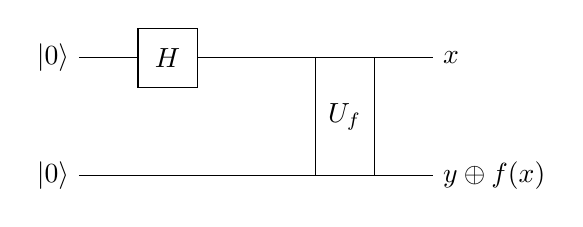
\begin{tikzpicture}[scale=1.5]
\draw (0,1) -- (3,1);
\draw (0,0) -- (3,0);
\node[left] at (0,1) {$|0\rangle$};
\node[left] at (0,0) {$|0\rangle$};
\draw[fill=white] (0.5,0.75) rectangle (1,1.25);
\node at (0.75,1) {$H$};
\draw[fill=white] (2,1) rectangle (2.5,0);
\node at (2.25,0.5) {$U_f$};
\node[right] at (3,1) {$x$};
\node[right] at (3,0) {$y \oplus f(x)$};
\end{tikzpicture}
\caption{Circuit diagram for $U_f|x,y\rangle = |x,y \oplus f(x)\rangle$ where the first qubit is in superposition and second qubit is $|0\rangle$}
\end{figure}

The algorithm's steps:
\begin{enumerate}
    \item Apply Hadamard gates to input state $|0\rangle|1\rangle$ to produce product state of superpositions
    \item Apply $U_f$ to that product state
    \item Apply Hadamard gate to first qubit only
\end{enumerate}

\begin{conceptbox}
Let's examine how $U_f$ acts on the computational basis states:
\[
U_f|00\rangle = |0, 0 \oplus f(0)\rangle = (1-f(0))|00\rangle + f(0)|01\rangle
\]

This result accounts for both possibilities where $0 \oplus f(0) = 0$ and $0 \oplus f(0) = 1$. To understand this:
\begin{itemize}
    \item If $f(0) = 0$, then $0 \oplus f(0) = 0 \oplus 0 = 0$ and:
    \[
    |0, 0 \oplus f(0)\rangle = (1-f(0))|00\rangle + f(0)|01\rangle = |00\rangle + (0)|01\rangle = |00\rangle
    \]
    \item If $f(0) = 1$, then $0 \oplus f(0) = 0 \oplus 1 = 1$ and:
    \[
    |0, 0 \oplus f(0)\rangle = (1-f(0))|00\rangle + f(0)|01\rangle = (0)|00\rangle + (1)|01\rangle = |01\rangle
    \]
\end{itemize}

Similar logic applies to the other basis states:
\begin{align*}
U_f|01\rangle &= |0, 1 \oplus f(0)\rangle = f(0)|00\rangle + (1-f(0))|01\rangle \\
U_f|10\rangle &= |1, 0 \oplus f(1)\rangle = (1-f(1))|10\rangle + f(1)|11\rangle \\
U_f|11\rangle &= |1, 1 \oplus f(1)\rangle = f(1)|10\rangle + (1-f(1))|11\rangle
\end{align*}
\end{conceptbox}

\begin{theorem}[Deutsch's Algorithm Output]
The final output state is:
\[
|\psi_{\text{out}}\rangle = \begin{cases}
(1-2f(0)

|0\rangle\oplus\left(\frac{|0\rangle - |1\rangle}{\sqrt{2}}\right) & \text{if } f(0) = f(1) \text{ (constant)} \\
\pm|1\rangle\oplus\left(\frac{|0\rangle - |1\rangle}{\sqrt{2}}\right) & \text{if } f(0) \neq f(1) \text{ (balanced)}
\end{cases}
\]
\end{theorem}

\subsection{Deutsch-Jozsa Algorithm}
\begin{definition}[Deutsch-Jozsa Algorithm]
A generalization of Deutsch's algorithm for functions with multiple input values. For $f(x)$ with $n$ input values:
\begin{itemize}
    \item \textbf{Constant}: Output is same for all input values $x$
    \item \textbf{Balanced}: $f(x) = 0$ for half inputs and $f(x) = 1$ for other half
\end{itemize}
\end{definition}

\begin{figure}[h]
    \centering
    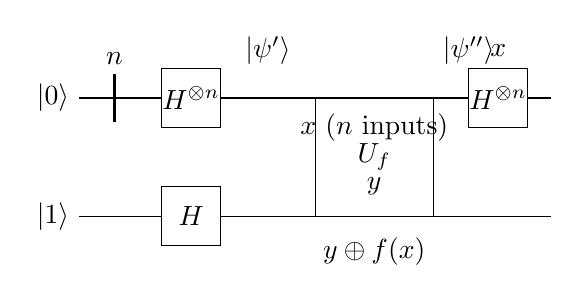
\begin{tikzpicture}[scale=1.5]
    % Lines
    \draw (0,1) -- (4,1);
    \draw (0,0) -- (4,0);
    
    % Initial states
    \node[left] at (0,1) {$|0\rangle$};
    \node[left] at (0,0) {$|1\rangle$};
    
    % n-qubit notation
    \draw[thick] (0.3,1.2) -- (0.3,0.8);
    \node[above] at (0.3,1.2) {$n$};
    
    % First H gates
    \draw[fill=white] (0.7,0.75) rectangle (1.2,1.25);
    \node at (0.95,1) {$H^{\otimes n}$};
    \draw[fill=white] (0.7,-0.25) rectangle (1.2,0.25);
    \node at (0.95,0) {$H$};
    
    % State labels
    \node at (1.6,1.4) {$|\psi'\rangle$};
    
    % Uf box
    \draw[fill=white] (2,1) rectangle (3,0);
    \node at (2.5,0.75) {$x$ ($n$ inputs)};
    \node at (2.5,0.5) {$U_f$};
    \node at (2.5,0.25) {$y$};
    
    % Output labels
    \node at (3.3,1.4) {$|\psi''\rangle$};
    \node at (2.5,-0.3) {$y \oplus f(x)$};
    
    % Final H gate
    \draw[fill=white] (3.3,0.75) rectangle (3.8,1.25);
    \node at (3.55,1) {$H^{\otimes n}$};
    
    % Output x label
    \node at (3.55,1.4) {$x$};
    \end{tikzpicture}
    \caption{Circuit diagram for the Deutsch-Jozsa algorithm showing the $n$-qubit input register and auxiliary qubit}
\end{figure}

\begin{theorem}[Measurement Results]
After measuring the $n$ input qubits in the final state:
\begin{itemize}
    \item If all qubits are 0: $f(x)$ is constant
    \item If at least one qubit is 1: $f(x)$ is balanced
\end{itemize}
\end{theorem}

\begin{example}[Constant Function]
For $f(x) = 1$ with two inputs:
\begin{enumerate}
    \item Initial state: $|\psi_{\text{in}}\rangle = |0\rangle|0\rangle|1\rangle$
    \item After Hadamard gates:
    \[
    |\psi_t\rangle = \frac{1}{2\sqrt{2}}(|000\rangle - |001\rangle + |010\rangle - |011\rangle + |100\rangle - |101\rangle + |110\rangle - |111\rangle)
    \]
    \item Final state after all operations:
    \[
    |\psi_{\text{out}}\rangle = -|00\rangle\left(\frac{|0\rangle - |1\rangle}{\sqrt{2}}\right)
    \]
    \item Measurement of first two qubits gives 00, confirming constant function
\end{enumerate}
\end{example}

\begin{example}[Balanced Function]
For $f(00) = f(01) = 0$, $f(10) = f(11) = 1$:
\begin{enumerate}
    \item Initial state: $|\psi_{\text{in}}\rangle = |0\rangle|0\rangle|1\rangle$
    \item After all operations:
    \[
    |\psi_{\text{out}}\rangle = |10\rangle\left(\frac{|0\rangle - |1\rangle}{\sqrt{2}}\right)
    \]
    \item Measurement of first two qubits gives 10, confirming balanced function
\end{enumerate}
\end{example}

\end{document}